% Default course lecture note template by asp 
\documentclass[letterpaper]{article}
\usepackage[utf8]{inputenc}
\usepackage[T1]{fontenc}
\usepackage[english]{babel}
\usepackage[top=3cm, bottom=3cm, left=3.85cm, right=3.85cm]{geometry}
\usepackage[onehalfspacing]{setspace}
\usepackage{hyperref}
\usepackage{amsmath,amsthm,amssymb,wasysym,fdsymbol,marvosym}
\usepackage{graphicx}
\usepackage[usenames,dvipsnames]{color}

\newtheoremstyle{xxx}
  {0pt}{1pt}
  {\color{BrickRed}}
  {0pt}
  {\bf}{.}{ }{}
\newtheoremstyle{yyy}
  {0pt}{1pt}
  {\color{OliveGreen}}
  {0pt}
  {\bf}{.}{ }{}
\newtheoremstyle{zzz}
  {0pt}{1pt}
  {\color{Blue}}
  {0pt}
  {\bf}{.}{ }{}
\newtheoremstyle{evil}
  {2pt}{2pt}
  {\color{red} \bf}
  {0pt}
  {\bf}{.}{ }{}

\theoremstyle{xxx}
\newtheorem{thrm}{Theorem}
\newtheorem{thrm-s}{Sanity Check}
\newtheorem{prop}{Proposition}
\theoremstyle{evil}
\newtheorem{warn}{Warning}
\newtheorem{evil}{Evil}
\theoremstyle{yyy}
\newtheorem{corl}{Corollary}
\newtheorem{lmma}{Lemma}
\theoremstyle{plain}
\newtheorem{expl}{Example}
\theoremstyle{zzz}
\newtheorem{defn}{Definition}

\newcommand{\notn}{\paragraph{Notation.}}
\newcommand{\recl}{\paragraph{Recall.}}
\newcommand{\rmrk}{\paragraph{Remark.}}
\newcommand{\note}{\paragraph{Note.}}

\newcommand{\ftwo}{\mathbb{F}_2}
\newcommand{\fttwo}{\mathbb{F}_{32}}
\newcommand{\binrep}[1]{\left\{#1\right\}}
\newcommand{\vc}[1]{\texttt{#1}} % volvelle character

\begin{document}

% Two-column title block
\begin{minipage}[b]{0.7\linewidth}
{\huge The Math Behind the Volvelles}
\end{minipage}
\begin{minipage}[b]{0.3\linewidth}
  \begin{flushright}
    Andrew Poelstra\\
    2021 December 6
  \end{flushright}
\end{minipage}
\\

% Actual content start
\section{Mathematical Preliminaries}

In this first section we give a crash course in field theory. Readers familiar
with this material should have no problem skipping or skimming this section,
at least up to Section \ref{sec:sss}.
Readers who are completely unfamiliar with this material are unlikely to be
able to follow the condensed exposition, and are encouraged to consult
standard algebra textbooks (e.g. the one by Dummit and Foote) or Wikipedia.

\subsection{Fields and $\ftwo$}
Consider the integers modulo 2. This is a set consisting of two equivalence
classes, the evens and the odds, which hereafter we will refer to as 0 and 1.
This set is a \textbf{field}, which means that when we define addition and
multiplication in the obvious way, it satisfies the following axioms:
\begin{enumerate}
\item The set is closed under addition; addition is associative, commutative,
has an identity element 0, and all elements have additive inverses. In other
words it is an \textbf{abelian group} under addition.
\item Similarly it is an abelian group under multiplication, with identity 1.
\item The \textbf{distributive law} holds, which means that $a(b + c)$ always
equals $ab + ac$.
\end{enumerate}

We refer to this field as $\ftwo$. For any field, we refer to its nonzero
elements as the \textbf{multiplicative group} of the field. We observe that
the multiplicative group of $\ftwo$ has only the identity element.

\subsection{Polynomial Rings}

Since $\ftwo$ has only two elements, it is hard to do interesting algebra on
it. But it is a fact that, by adjoining a formal symbol $x$ to a field, we
can obtain a much bigger (in fact, countably infinite) set of \emph{polynomials}
in $\ftwo$. We denote this set $\ftwo[x]$ and call it the \textbf{polynomial
ring} of the field.

Formally, the set of polynomials is defined as

\[ \left\{ \sum_{i=0}^n a_ix^i : n\in\mathbb{N}\cup\{0\}, a_i\in \ftwo  \right\} \]

A ring, for our purposes, is defined the same way as a field except that we do
not require multiplication to be invertible. It is easy to check that the
polynomial ring, endowed with addition and multiplication in the obvious ways,
is in fact a ring.

For a polynomial of the form $\sum_{i=0}^n a_ix^i$ we refer to $n$ as the
\textbf{degree} of the polynomial. It is an elementary fact that the product
of polynomials has degree equal to the sum of the degrees of the factors.

We refer to polynomials of degree 0 is \textbf{constant polynomials}. It is
also a fact that a polynomial has a multiplicative inverse, i.e. it is a
\textbf{unit}, if and only if it is constant.

If a polynomial $r$ can be written as the product of two polynomials as $r=pq$,
where neither $p$ nor $q$ are units (degree 0) we say that $r$ is
\textbf{irreducible}.

\subsection{Quotient Fields}

Just like we can consider the integers modulo some integer $n$, thus obtaining
$n$ equivalence classes which inherit (roughly) the original ring structure of
the integers, we can consider a polynomial ring modulo some polynomial $p$. In
this case, we will get $m^n$ equivalence classes, where $m$ is the number of
elements in the underlying field and $n$ is the degree of the polynomial. For
our purposes $m$ is always 2, so we get $2^n$ elements.

We call the set of equivalence classes a \textbf{quotient ring}, and its addition
and multiplication are defined in the obvious way.

Just like in the integer case, if our polynomial $p$ can be factored into
nonconstant polynomials as $p=p_1p_2$, their images in the quotient ring will
be nonzero but satisfy $p_1p_2 = 0$. In other words they are \textbf{zero
divisors} and imply that multiplication in the ring is not invertible.

We do not like zero divisors, so from here on out we will be sure to mod out
our polynomial ring only by irreducible polynomials. It is a fact that the
resulting quotient ring will then be a field, and we term it a \textbf{quotient
field}. It is a fact that $x^5 + x^3 + 1$ is irreducible in $\ftwo$, so that
$\ftwo/(x^5 + x^3 + 1)$ is a quotient field with 32 elements.

In this field the object $x$ is a field element with a distinct identity and
algebraic properties, so we rename it $\alpha$ to preserve the symbol $x$ to
be an indeterminate used for writing polynomials.

It is a fact that, for this specific polynomial, that $\alpha$ is a
\textbf{generator} of the quotient field, meaning that the field in its entirety
is equal to
\[ \left\{ \alpha^i : i \in \{0,1,\ldots,30\} \right\} \]
and zero.

We observe that the order of the multiplicative group is 31, a prime, and therefore
every element of the group except 1 is a generator of the group. Furthermore there
are no nontrivial proper subgroups. These are an elementary facts of group theory.

We refer to this new field as $\fttwo$. It is fact of field theory that all
groups with 32 elements are isomorphic to this one, which justifies the name.
But bear in mind that, for our purposes, the field was constructed as $\ftwo[x]/
(x^5 + x^3 + 1)$ and has a distinguished generator $\alpha$ which is a root
of that polynomial.

\subsection{Vector Spaces}

We observe that $\fttwo$ is a \textbf{vector space} over $\ftwo$. A vector
space $V$ over a field $\mathbb{F}$ is defined by the following axioms:

\begin{enumerate}
\item $V$ is an abelian group with operation $+$ and identity $0_V$.
\item $(a + b)v = av + bv$ and $a(u + v) = au + av$ for all $a,b\in \mathbb{F}$ and
$u,v\in V$.
\end{enumerate}

We refer to a finite sum of the form $\sum_i f_iv_i$ with $f_i\in \mathbb{F}$ and
$v_i\in V$ as a \textbf{linear combination}. We observe that every element
of $\fttwo$ is a linear combination of the elements $\{1,\alpha,\alpha^2,
\alpha^3,\alpha^4\}$, and that no smaller set of elements has this property.
We call such a set a \textbf{basis} for $\fttwo$.

\subsection{Lagrange Interpolation and Shamir's Secret Sharing\label{sec:sss}}

Let $\mathbb{F}$ be a field and $p$ a polynomial of degree $n$ in $\mathbb{F}[x]$. It is a
standard theorem of algebra that $p$'s value on all points of $\mathbb{F}$ is
implied by its values on any $n+1$ distinct points.

As discovered by Edward Waring in 1779, and later by Joseph-Louis Lagrange
in 1795\footnote{citation: Wikipedia}, it is actually possible to compute
the value of a polynomial at a field element $x$ explicitly in terms of
its values at $n$ given distinct points $x_i$.

Specifically, suppose that $p(x_i) = y_i$. Then
\begin{equation}
 p(x) = \sum_{i=1}^{n+1} y_i \ell_i(x) \label{eq:linterp}
\end{equation}
where $\ell_i$ is determined entirely by the $x_i$'s, as
\[ \ell_i(x) = \prod_{j\neq i} \frac{x - x_j}{x_i - x_j} \]

There are several very interesting observations to be made here:
\begin{enumerate}
\item First, for a fixed set of $x_i$'s, we see that the vector space of
$n$-degree polynomials over $\mathbb{F}$ is spanned by the set $\{\ell_i(x)\}$. Since
there are $n+1$ polynomials and this space has dimension $n+1$ (an obvious
basis for it is $\{ 1,x,x^2,\ldots,x^n\}$), this means that the set
$\{\ell_i(x)\}_i$ forms a basis for this space.
\item Further, these basis polynomials satisfy the equality
$\sum_i \ell_i(x) = 1$. (One way to see this is by using equation
\eqref{eq:linterp} to interpolate the constant one polynomial.)

This means that equation \eqref{eq:linterp} is an \textbf{affine
combination} of the $y_i$'s, a strengthening of the familiar notion
of linear combination. This property will become important, as we
will see.
\item If we further fix $x$, we see that knowing $p$'s evaluation at
every $x_i$ is sufficient to determine $p(x)$, while knowing any fewer
evaluations provides zero information about $x$: suppose for example
that $y_n$ is unknown. Then by a suitable choice of $y_n$ in \eqref{eq:linterp}
we can cause $p(x)$ to take any of the $|\mathbb{F}|$ possible values.
\end{enumerate}

Putting these facts together, we obtain \textbf{Shamir's Secret Sharing
Scheme} (SSSS) for splitting a secret element of $\mathbb{F}$ into up to $|\mathbb{F}|-1$
shares, such that a fixed threshold number $k$ of them are sufficient
to reconstruct the secret:

\begin{enumerate}
\item First, fix an index $s\in \mathbb{F}$ to be the secret index.
\item Generate a random $(k-1)$-degree polynomial $p$ by choosing $k$
random values and assigning them to be the evaluation of $p$ at specific
points $x_i\in \mathbb{F}$.

(If the secret is known beforehand, then fix $p(s)$ to be the secret
and generate $k-1$ other evaluations of $p$. randomly.)
\item Distribute the points $x_i$ along with their evaluations $p(x_i)$
to multiple parties.
\item Then if any $k$ of them come together, they can use equation
\eqref{eq:linterp} to reconstruct the secret $p(s)$.
\end{enumerate}

We call the $k$ randomly generated values \textbf{initial shares} and
every other evaluation of $p$ a \textbf{derived share}.

There are several interesting observations here:
\begin{itemize}
\item If we have a sequence $F_x = \{f_i\}$ of elements of $\mathbb{F}$, we can use
SSSS in parallel on all of them, choosing independently random polynomials
$\{p_i\}$ and distributing the sequence $\{p_i(x)\}$ along with the evaluation
point $x$.
\item If, for some particular $i$, $f_i$ is constant across our $k$ initial
shares $F_{x_1},\ldots,F_{x_k}$, Lagrange interpolation will cause the same
constant to appear in the same position for all derived shares. So you can
have, say, a fixed header on all of your shares which will be preserved by
the secret-sharing mechanism.
\item Similarly, for some particular $i$, you set $f_i=x$, i.e. you encode the
evaluation point in a fixed place in your sequence, then Lagrange interpolation
will interpolate the polynomial $p(x) = x$ here and place the correct value
of $x$ in the correct place for all shares.
\item Going even further, suppose for each initial share $F_x=\{f_i\}$, some fixed
affine relation holds among the $f_i$'s, e.g.
\[ \sum_i \alpha_i f_i = \beta \]
for fixed $\beta,\alpha_i\in \mathbb{F}$. Then this fixed affine relation
\emph{will continue to hold for all derived shares}!

This is not immediately obvious but can be shown by direct computation and
using the fact that Lagrange interpolation is an affine combination of $f_i$'s.
\end{itemize}

This fact is so important that we term it the \textbf{Fundamental Theorem of
Computing SSSS with Volvelles}. The Fundamental Theorem implies that if we
apply any checksum derived from a linear code (or a linear code plus a
constant) to our initial shares, that the derived shares will automatically
be checksummed as well.

For more information about volvelles, see the next two sections.

\subsection{The Bech32 Alphabet}

The previous section indicated that if $\beta\in\fttwo$, then we can write
\[ \beta = b_4\alpha^4 + b_3\alpha^3 + b_2\alpha^2 + b_1\alpha + b_0 \]
where each $b_i\in\{0, 1\}$. We can therefore encode $\beta$ as a 5-bit
number by directly encoding the bits $b_i$. Alternately, since there are
only 32 such $\beta$s, we assign them all alphanumeric symbols, with four
symbols to spare. This is the premise behind the \textbf{bech32 alphabet},
defined in BIP 173, and reproduced on the following page.

In addition to the bech32 alphabet, which uses Latin characters, we also use
an alternate alphabet using Greek letters and various symbols.

We have ordered all the symbols in three ways -- $\alpha$betically,
alphabetically, and by their ``numeric'' binary value. These three
representations are useful in different contexts:
\begin{enumerate}
\item Representing elements as a power of $\alpha$ makes multiplication
very easy, since multiplication is just addition mod 31 in the exponent.

This is how our multiplication wheel can be implemented as a slide rule.
\item Representing alphabetically makes it easy for humans to scan and sort.
\item Representing in binary is how the elements are typically stored in
computers, can be used to convert data from other encodings. Addition is
simply xor in this format.
\end{enumerate}

\clearpage
~\\~\\~\\~\\ % vertical centering

% Ordered by power
\begin{minipage}[b]{0.3\linewidth}
\begin{center}
\begin{tabular}{|cccc|}
\hline
Q & $\times$   & - & 00000 \\
P & $\aleph$   & $\alpha^0$ & 00001 \\
Z & $\alpha$   & $\alpha^1$ & 00010 \\
Y & $\Gamma$   & $\alpha^2$ & 00100 \\
G & $\Theta$   & $\alpha^3$ & 01000 \\
S & $\Psi$     & $\alpha^4$ & 10000 \\
F & $\Lambda$  & $\alpha^5$ & 01001 \\
J & @          & $\alpha^6$ & 10010 \\
D & $\rho$     & $\alpha^7$ & 01101 \\
6 & \textdagger& $\alpha^8$ & 11010 \\
A & $\P$       & $\alpha^9$ & 11101 \\
N & \#         & $\alpha^{10}$ & 10011 \\
0 & $\Phi$     & $\alpha^{11}$ & 01111 \\
7 & $\blacklozenge$ & $\alpha^{12}$ & 11110 \\
4 & $\cent$    & $\alpha^{13}$ & 10101 \\
R & $\beta$    & $\alpha^{14}$ & 00011 \\
X & $\epsilon$ & $\alpha^{15}$ & 00110 \\
V & $\Pi$      & $\alpha^{16}$ & 01100 \\
C & \textcurrency & $\alpha^{17}$ & 11000 \\
E & $\oplus$   & $\alpha^{18}$ & 11001 \\
M & \textdaggerdbl & $\alpha^{19}$ & 11011 \\
L & $\varheartsuit$ & $\alpha^{20}$ & 11111 \\
H & \EUR       & $\alpha^{21}$ & 10111 \\
8 & $\eta$     & $\alpha^{22}$ & 00111 \\
W & $\Sigma$   & $\alpha^{23}$ & 01110 \\
U & $\S$       & $\alpha^{24}$ & 11100 \\
3 & $\Omega$   & $\alpha^{25}$ & 10001 \\
T & $\Xi$      & $\alpha^{26}$ & 01011 \\
K & \yen       & $\alpha^{27}$ & 10110 \\
9 & $\Delta$   & $\alpha^{28}$ & 00101 \\
2 & $\mu$      & $\alpha^{29}$ & 01010 \\
5 & \%         & $\alpha^{30}$ & 10100 \\
\hline
\end{tabular}
\end{center}
\end{minipage}
% Ordered by alphabet
\begin{minipage}[b]{0.3\linewidth}
\begin{center}
\begin{tabular}{|ccc|}
\hline
A & $\alpha^9$ & 11101 \\
C & $\alpha^{17}$ & 11000 \\
D & $\alpha^7$ & 01101 \\
E & $\alpha^{18}$ & 11001 \\
F & $\alpha^5$ & 01001 \\
G & $\alpha^3$ & 01000 \\
H & $\alpha^{21}$ & 10111 \\
J & $\alpha^6$ & 10010 \\
K & $\alpha^{27}$ & 10110 \\
L & $\alpha^{20}$ & 11111 \\
M & $\alpha^{19}$ & 11011 \\
N & $\alpha^{10}$ & 10011 \\
P & $\alpha^0$ & 00001 \\
Q & - & 00000 \\
R & $\alpha^{14}$ & 00011 \\
S & $\alpha^4$ & 10000 \\
T & $\alpha^{26}$ & 01011 \\
U & $\alpha^{24}$ & 11100 \\
V & $\alpha^{16}$ & 01100 \\
W & $\alpha^{23}$ & 01110 \\
X & $\alpha^{15}$ & 00110 \\
Y & $\alpha^2$ & 00100 \\
Z & $\alpha^1$ & 00010 \\
0 & $\alpha^{11}$ & 01111 \\
2 & $\alpha^{29}$ & 01010 \\
3 & $\alpha^{25}$ & 10001 \\
4 & $\alpha^{13}$ & 10101 \\
5 & $\alpha^{30}$ & 10100 \\
6 & $\alpha^8$ & 11010 \\
7 & $\alpha^{12}$ & 11110 \\
8 & $\alpha^{22}$ & 00111 \\
9 & $\alpha^{28}$ & 00101 \\
\hline
\end{tabular}
\end{center}
\end{minipage}
% Ordered by binary
\begin{minipage}[b]{0.3\linewidth}
\begin{center}
\begin{tabular}{|ccc|}
\hline
Q & - & 00000 \\
P & $\alpha^0$ & 00001 \\
Z & $\alpha^1$ & 00010 \\
R & $\alpha^{14}$ & 00011 \\
Y & $\alpha^2$ & 00100 \\
9 & $\alpha^{28}$ & 00101 \\
X & $\alpha^{15}$ & 00110 \\
8 & $\alpha^{22}$ & 00111 \\
G & $\alpha^3$ & 01000 \\
F & $\alpha^5$ & 01001 \\
2 & $\alpha^{29}$ & 01010 \\
T & $\alpha^{26}$ & 01011 \\
V & $\alpha^{16}$ & 01100 \\
D & $\alpha^7$ & 01101 \\
W & $\alpha^{23}$ & 01110 \\
0 & $\alpha^{11}$ & 01111 \\
S & $\alpha^4$ & 10000 \\
3 & $\alpha^{25}$ & 10001 \\
J & $\alpha^6$ & 10010 \\
N & $\alpha^{10}$ & 10011 \\
5 & $\alpha^{30}$ & 10100 \\
4 & $\alpha^{13}$ & 10101 \\
K & $\alpha^{27}$ & 10110 \\
H & $\alpha^{21}$ & 10111 \\
C & $\alpha^{17}$ & 11000 \\
E & $\alpha^{18}$ & 11001 \\
6 & $\alpha^8$ & 11010 \\
M & $\alpha^{19}$ & 11011 \\
U & $\alpha^{24}$ & 11100 \\
A & $\alpha^9$ & 11101 \\
7 & $\alpha^{12}$ & 11110 \\
L & $\alpha^{20}$ & 11111 \\
\hline
\end{tabular}
\end{center}
\end{minipage}

\clearpage

\subsection{The Addition Volvelle}

Volvelles, or slide charts, are computers constructed by two sheets of paper, cut
into circles and affixed at the center so that they are able to rotate relative
to each other.

\begin{center} 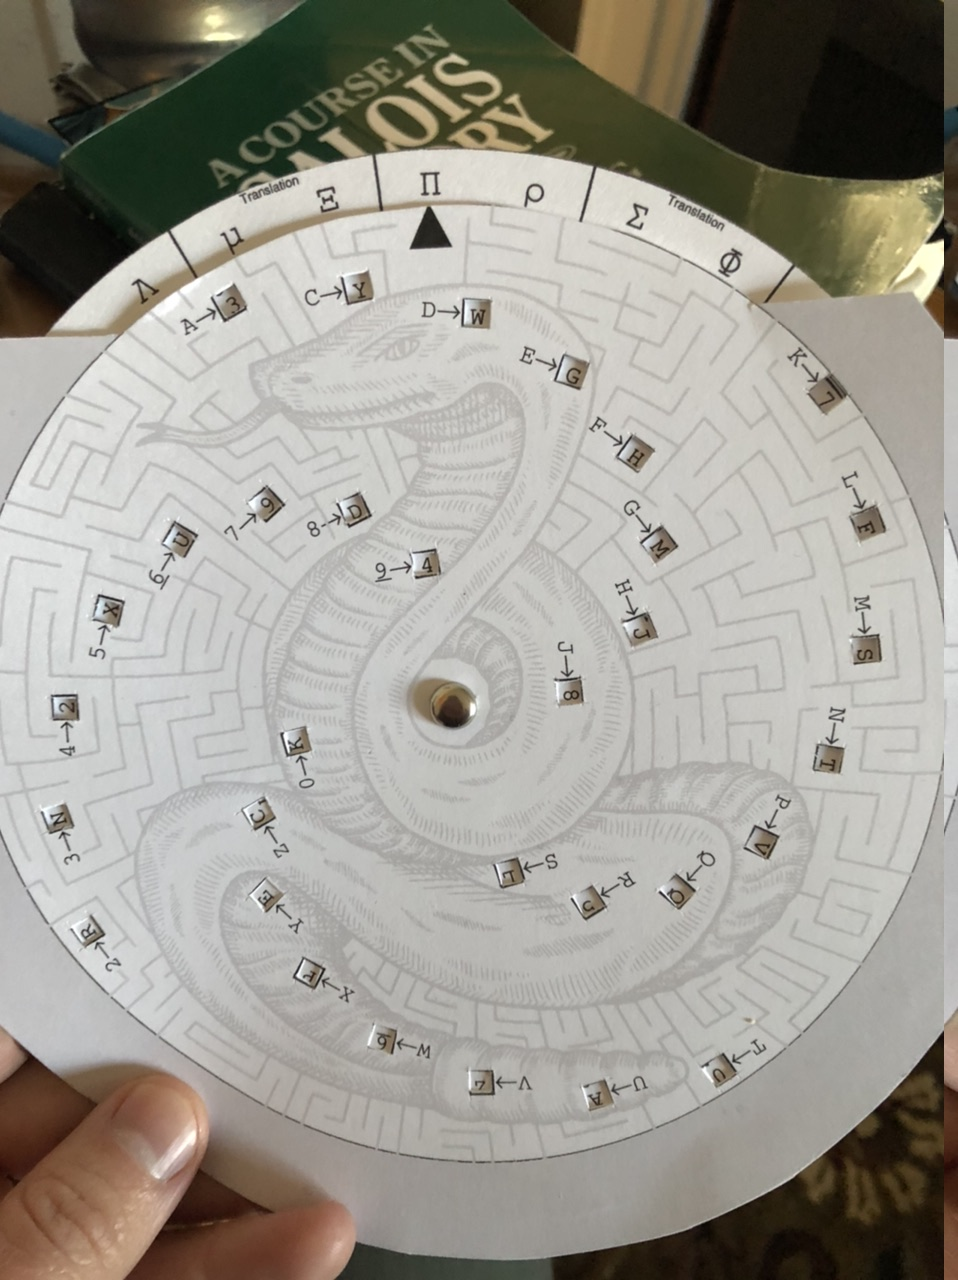
\includegraphics[scale=0.35]{volvelle.jpeg} \end{center}

The top sheet has holes cut into it, selectively revealing data printed on the
bottom sheet, depending on the rotation. The top sheet has a pointer used to
index the data being revealed.

\paragraph{The Addition Volvelle.} We have provided one volvelle, which computes
addition in $\fttwo$. By setting the pointer to some value $x$, and looking at
the window labeled $y\to$, the value $x+y$ will be revealed. It is instructive
to observe that the expected symmetries are there: $x+y=y+x$, $x+x=Q$, $x+Q=x$,
etc.

\paragraph{Volvelles and Algebraic Structure.} Our volvelle has 32 holes cut
in the face, corresponding to the 32 bech32 characters. If all 32 positions
of the volvelle revealed distinct locations on the bottom wheel, it would
require symbols to be printed on the bottom wheel in 1024 positions. If there
were algebraic structure relating the results of different volvelle positions,
we could reduce this number.

We will return to this idea in the next section, about slide rules, but for now
we simply observe that we did \textbf{not} reduce the number of symbols from
the maximum 1024.

Why not? Well, observe that the way to reduce symbols is to have two windows at
the same radius from the center of the volvelle. Then on the bottom sheet, a
single circle of values would provide the revealed symbols for both windows.
Let's say that one window is labeled $x\to$, and the other labeled $y\to$. Then
since the windows are at a fixed angle $\theta$ from each other (being printed
on the same solid sheet of paper), we would require the bottom circle of values
to satisify
\[ \textnormal{for all } z\in\fttwo:\qquad x + z \textnormal{ and } y+z \textnormal{ are at angle $\theta$ to each other} \]
Now, $x+z$ and $y+z$ differ by the fixed quantity $x+y$ (recall we are in
characteristic 2), so this can be restated as
\[ \textnormal{for all } z\in\fttwo:\qquad z \textnormal{ and } z+(x+y) \textnormal{ are at angle $\theta$ to each other} \]
Then observing that $(x+y) + (x+y) = 0$, two applications of the above equation
give us
\[ \textnormal{for all } z\in\fttwo:\qquad z \textnormal{ is at angle $2\theta$ from itself} \]
It is now clear that if we either need to repeat characters (defeating the goal
of reducing the amount of symbols on the bottom wheel) or have $\theta=180^\circ$.

Okay, so perhaps we can get a 50\% reduction in density for the bottom wheel, by
setting $\theta=180^\circ$ and having the windows on opposite sides of the top
wheel be at the same radius and use the same set of bottom-wheel symbols.

Let's play this out. Take, for example, the \vc{A} and \vc{T} windows on the
addition volvelle. These differ by \vc{K}, so we require that on the bottom
wheel, symbols at this radius differ from their opposite symbol by \vc{K}.
If the top wheel is pointing at some symbol $a$, and we turn it $180^\circ$
to $b$, we have simply exchanged the values in these windows, i.e. added
\vc{K} to both. But this implies that $a+b=\vc{K}$.

In other words, for this compression to work, we need every pair of opposing
symbols to add to \vc{K}; i.e. we need to take the sixteen 2-element cosets
obtained by modding out by \vc{K} and then order the symbols so that each
coset's members appear opposite each other.

It can be seen, by modding out by every possible symbol, and trying various
orderings of the resulting cosets, that no such choice will lead to a
``natural'' ordering\footnote{There are 16 cosets, so $15\approxeq2^{40}$
different arrangements around a circle. Then you can exchange the members
in each coset, for another $2^{15}$ possibilities. So an exhaustive search
would require about $2^{55}$ work. I did not do an exhaustive search, so I
may be wrong in claiming that ``no such choice'' works. But I spent several
hours starting from random permutations and then looking for local optima
and never got very close. My measure of ``naturalness'' was to take the
distance $d$ between each character and its alphanumeric successor, and to
sum all the $2^d$s.}. This means that to get this compression, we'd need
to reorder the wheel such that users wouldn't know which direction to spin
to find a desired symbol, and the resulting harm to usability would exceed
the benefit of having larger windows.

If this argument was too abstract, take the addition volvelle and spin it to
\vc{C} (one right of \vc{A}) and look at the symbols in the \vc{A} and \vc{T}
windows. Then spin it $180^\circ$ to \vc{U} (one right of \vc{T}) and look
at the same symbols. You will see different symbols. For this scheme to work,
they would need to be the same symbols. Ergo, we'd have to reorder the symbols
in a confusing order to make this work.

(By the way, this \emph{could} be made to work if we rearranged our mapping
between bech32 symbols and $\fttwo$ objects so that the \vc{K}-cosets, or
whatever, were naturally ordered. But deviating from the bech32 spec in this
way, for such a minor benefit in volvelle layout, doesn't seem worth the
potential confusion/incompatibility between the schemes.)

\subsection{The Multiplication-Translation Slide Rule}

\paragraph{Multiplication.}
While the addition volvelle could not be re-arranged to reduce the number of
symbols beyond 1024, let's consider the second operation we might like to do:
\emph{multiplication}.

For reasons that we will describe later, when multiplying in $\fttwo$ it turns
out that we want to use the alternate symbol alphabet rather than the bech32
alphabet. We also don't care so much about multiplication by zero, which always
results in zero, which we can tell the user rather than putting it into a
volvelle.

Now, we have 31 nonzero elements, so a volvelle would naively have $31^2=961$
entries. Can we do better? Using the same reasoning as with the addition volvelle,
if we wanted two windows $x\to$ and $y\to$ to share a radius, we'd need that
\[ \textnormal{for all } z\in\fttwo:\qquad xz \textnormal{ and } yz \textnormal{ are at angle $\theta$ to each other} \]
We have a group under multiplication with 31 elements in it. It is then a fact
that if we choose any element $\alpha\in\fttwo^*$ except 1, that $\alpha$
\textbf{generates} the group. Meaning that every element $z$, including 1,
can be written as $z=\alpha^{i_z}$ where $i_z$ is some integer modulo 31. So we
may write
\[ \textnormal{for all } \alpha^{i_z}\in\fttwo:\qquad \alpha^{i_x}\alpha^{i_z} = \alpha^{i_x+i_z} \textnormal{ and } \alpha^{i_y}\alpha^{i_z} = \alpha^{i_y+i_z} \textnormal{ are at angle $\theta$ to each other} \]

By squinting at this for a moment, you can observe that if $\theta$ is one 31th
of a full rotation, and we make sure that each $\alpha^i$ on the front wheel is
followed by $\alpha^{i+1}$, then \emph{every single window can have the same
radius}. In fact, we don't need windows, since the bottom wheel now has only a
single circle of symbols, all of which are always visible.

This is the intuition behind the \textbf{multiplication wheel}, which is actually
a circular slide wheel:

FIXME put an image here

\paragraph{Translation.} There are actually two kinds of multiplication that
we might want to do: symbol-by-symbol multiplication and symbol-by-bech32-character
multiplication. The latter we refer to as \textbf{translation}.

Algebraically, multiplication and translation are identical, of course. But in
practice, multiplication is used to combine $k=2$ Lagrange basis polynomials
(encoded as symbols) to get $k>2$ basis polynomials (also symbols).
Meanwhile transalation is used to multiple the basis polynomials (symbols) by
share values (characters) to get translated shares (characters).

Since translation is identical to multiplication, we might hope that we could
construct a translation slide rule by simply relabelling the multiplication
slide rule. Indeed, we could do this by changing the inner wheel to use
bech32 characters rather than symbols. Then to translate a character $c$ by
a symbol $\sigma$, the user would turn the wheel to point to $c$, look for
$\sigma$, and find what it points to.

However, in practice this is a pretty awkward setup, for two reasons:
\begin{itemize}
\item Again, because the correspondence between bech32 characters and $\fttwo$
does not have any algebraic structure, ordering the characters by increasing
powers of $\alpha$ results in an unintuitive ordering.

We have chosen to just live with this problem. All the characters are visible
at the same time, so it isn't nearly as a bad a usability burden as it would've
been with a volvelle.
\item Since zero (\vc{Q}) is a valid share value, we actually do need to think
about multiplication by 0.

In contrast, zero would not be valid Lagrange basis polynomial, unless the user
tried to input the \vc{S} share, which the Recovery slide rule (see next section)
won't let her do.

We solve this by just printing $\vc{Q}\leftrightarrow\vc{Q}$ on the front of
the slide rule.
\item Most importantly, under normal usage, a user has a single symbol $\sigma$
which she wants to translate the 48+ characters of a share by. If she had to
rotate the wheel to every symbol and then look up $\sigma$ again, this would
be tiring and error-prone.

It would be better if she could just turn the wheel to $\sigma$ and then look
up every character.
\end{itemize}

This seems physically impossible, since the wheel pointer points to a symbol
on the outer wheel, which uses the output (bech32) alphabet. However, Russell
noticed that if we simply glue the Translation wheel to the back of the
Multiplication wheel, with the symbol ordering reversed, the user can move
the pointer on the \emph{back} of the wheel and then do lookups on the
\emph{front}.

Of course, we are mathematicians, so while we have brass fasteners, we have
no glue. So the actual assembly method is to print both sides attached to
each other, then fold them together. We then have two slide rules, whose
top and bottom wheels are now the ``outer'' and ``inner'' wheels, and which
are on opposite sides of the same pages.

FIXME put an image here

\subsection{The Recovery Slide Chart}

There is one remaining paper computer to design. This one is the \textbf{Recovery
wheel}, which computes Lagrange basis polynomials, evaluated at \vc{S}. That is,
it computes the map
\[ (p, r) \mapsto \frac{r + S}{r + p} = \frac{r + S}{r + S + p + S} \eqqcolon \frac{\hat{r}}{\hat{r}+\hat{p}} = \frac{1}{1 + \hat{p}/\hat{r}} \]
(where $\hat{c}\coloneqq c+\vc{S}$ is just a relabeling of our character set).

The idea is that the user would turn the wheel so that the pointer points at
share index $p$, looks on the wheel for the arrow labeled $r$, and the resulting
symbol is the Lagrange basis polynomial. We notice that the result is undefined
when $r = p$, which corresponds to the case when you are trying to use the same
share twice, which makes intuitive sense.

Here $p$ and $r$ are both bech32 characters and the output is a symbol.

Now, as before we may write $\hat{p}=\alpha^{i_{\hat{p}}}$ and
$\hat{r}=\alpha^{i_{\hat{r}}}$, where $\alpha$ is a generator of our multiplicative
group. Then we have
\[ (p, r) \mapsto \left[ 1 + \alpha^{i_{\hat{p}} - i_{\hat{r}}} \right]^{-1} \]

The addition of 1 and the multiplicative inversion can be accomplished by more
relabeling, and the fact that we have a difference rather than sum in the exponent
of $\alpha$ can be accomodated by reversing the direction of our arrows relative
to the arrows on the multiplication wheel. Putting it all together, to get a
recovery slide rule, we
\begin{enumerate}
\item Reverse the arrows in our multiplication slide rule, as we are doing
division rather than multiplication.
\item Apply $x\mapsto x+\vc{S}$ to the inputs (which are now both on the bottom
wheel, so we can permute them independently of the outputs), and
$x\mapsto[1+x]^{-1}$ to the output (which is on the top wheel).
\end{enumerate}

FIXME put an image here

Finally, we observe that, if we center our slide rule on the $\alpha^0$ output
slot (the one with the pointer on it, rather than a symbol), looking $j$ positions
to the left and right we have the values
\[ \left[ 1 + \alpha^{-j} \right]^{-1} \textnormal{ and } \left[ 1 + \alpha^j \right]^{-1}  \]
and it can be computed directly that these sum to 1.
In fact, this is exactly the relation between pairs of Lagrange basis polynomials
for the case $k=2$. (There are only two of them, and they add up to one because
Lagrange basis polynomials form affine sets.) So we can draw horizontal lines
between these pairs, making the wheel visuall distinct from the other wheels and
also guiding the user in the $k=2$ case\footnote{Russell's reasoning for these
lines, which made sense to me when I first heard it, was that to look up these
basis polynomials, you turn to one symbol and look up the other; then turn to
the other and look up the symbol. So by some sort of symmetry of turning these
pairs all have to be opposite each other.

I'm not sure I see the symmetry he was referring to, but there is a simpler
algebraic reason: when you exchange $r$ and $p$, as you do when computing the
two Lagrange basis polynomials for the $k=2$ case, you replace $\hat{r}/\hat{p}$
with its reciprocal, which is the same as mirroring it over the $\alpha^0$
position on a slide rule. Then the fact that these add to 1 is just a restatement
of the fact that Lagrange basis polynomials form an affine set.

Is there a ``deeper'' reason this all works out?}


\paragraph{The two alphabets.}
Now that we have all four of our paper computers defined,
we can see the justification for having two alphabets: both share creation and
and secret recovery are implemented as Lagrange interpolation using Equation
\eqref{eq:linterp} on page \pageref{eq:linterp}. In that equation, we are performing
a linear combination of $y_i$ values, which are secret shares encoded as bech32
characters. These values are exclusively multiplied by Lagrange basis polynomials,
which are always products of terms of the form $(x + y)/(x + z)$.

The process then, to do Lagrange interpolation, is to determine the $\ell_i(x)$
polynomial evaluated at the target share $x$ (the share to create, or $S$ in the case
of recovery), which can be done either using lookup tables or by finding component
symbols on the Recovery Volvelle and multiplying them together using the Multiplication
Wheel. Next, multiply each share $y_i$ by the resulting $\ell_i(x)$, using the Translation
Volvelle, and add them together using the Addition Volvelle.

In short, the bech32 alphabet is used for share values and share indices (which must
use the same alphabet since the index is encoded in the share itself) while the
symbol alphabet is used for Lagrange basis polynomials and their factors. The user
never needs to add basis polynomials and never needs to multiply share values, so
providing this capability would serve only to enable wrong turns.

Unfortunately, it is still possible (and not difficult) for the user to confuse
share values and share indices. I don't believe there is any way to avoid this.

\subsection{BCH Codes}

The final preliminary we need is that of a \textbf{BCH code}. There is a
rich and enormous theory underlying BCH codes, and linear codes in general,
but we will take an operationalist point of view and summarize just the facts
that we need:

An \textbf{error-correcting code} is a mapping from a set of raw data, called
\textbf{messages} into a larger set of \textbf{codewords} which have
some extra algebraic structure. In particular, between every pair of
codewords there is a minimum \textbf{distance}, which measures the
number of characters at which the two codewords differ.

Since all codewords differ by at least the minimum distance $d$, if there
are at most $d-1$ errors in a codeword, the result is guaranteed not to
be a valid codeword, and to be detected as an error pattern. If there are fewer
than $d/2$ errors, the correct codeword is uniquely determined by being
the closest codeword to the error pattern, which means that this many
errors can actually be corrected.

A \textbf{BCH code} is a specific type of error-correcting code. In a BCH
code, codewords are constructed by encoding data as the coefficients of a
large polynomial, then affixing some number of \textbf{checksum characters}.
The checksum characters are chosen such that the resulting polynomial is in
a specific residue class modulo a \textbf{generator polynomial} $G(x)$.

Given a potential codeword, there is a unique minimum-degree polynomial
equivalent to this codeword modulo $G(x)$, which can be found by modular
reduction. We refer to this reduced polynomial as the \textbf{reside}
of the codeword.

There are several properties of a BCH code that we will need:
\begin{itemize}
\item The \textbf{degree} of the code is the degree the roots of its
generator polynomial. (Since the generator polynomial is not, in general, irreducible,
this is \emph{not} the degree of the generator polynomial.)

The degree of our BCH code, and that of bech32, is 2. Degree-1 BCH codes are
called \textbf{Reed-Solomon codes}.

\item The \textbf{length} of the code is how long a coded message can be
(including the checksum!) for the code to retain its error-correcting
properties.

The length $\ell$ can be computed as the smallest polynomial of the form
$x^\ell - x$ that the generator divides. It is then clear that if you have a
message of this length, that the $\ell$th character will be interpreted
as the coefficient of $x^{\ell-1} \equiv 1$ mod $G(x)$, meaning that it
will just mask your first character rather than being checksummed
independently.

The length of our code is 93. The length of bech32 is 1023 (although through
an exhaustive search, it was found to have better error detection properties
than the algebra would suggest, up to length 71).

This means that you cannot encode messages longer than 80 characters (six
character header plus 370 data bits) using this checksum! You must split
your data and use multiple checksums.

\item The $m$-value is the specific residue that all codewords must 
must have. All $m$ values are equivalent, in the sense that it is easy
to convert from one $m$ value to another (simply add the difference to
the checksum characters, modulo $G(x)$).

But $m=0$ has the particularly bad property that any codeword can be extended
by addition of an arbitrary number of 0s to get another valid codeword. (This
highlights the fact that BCH codes are designed to handle only \emph{substitution}
or \emph{erasure} errors, not insertions or deletions.) Other small values of
$m$ have similar issues; bech32 was originally defined to have $m=1$ but later
needed to be modified to bech32m for this reason. bech32m uses a large random
$m$ instead.

On the other hand, $m=0$ makes a BCH code a \textbf{linear code}, and brings
with it a ton of algebraic properties which are needed for analysis, so this
is what is used in the literature.

In practice it is common to use a string of all-bits-one for $m$. For our code,
we chose characters which spell out \vc{SECRETSHARE32}.

\item The \textbf{checksum length} is the number of extra characters that
need to be added to a string to ensure that it has the correct residue.
This value \emph{is} the degree of the generator polynomial.
\end{itemize}

We will return to BCH codes in the main text, when we discuss the Checksum
Worksheet and the properties of BCH codes which make them compatible with
Shamir's Secret Sharing.

\section{The Checksum}

We now get into the meat of the document, where we descibe how the actual
user processes are implemented. We start with the checksum.

\subsection{The Math}
Our checksum is defined by a BCH code with generator polynomial
\begin{align*}
    G(x) = x^{13}
        &+ \binrep{31}x^{12} + \binrep{5}x^{11} + \binrep{3}x^{10} + \binrep{28}x^9 + \binrep{0}x^8 + \binrep{31}x^7\\
        &+ \binrep{31}x^6 + \binrep{31}x^5 + \binrep{9}x^4 + \binrep{5}x^3 + \binrep{30}x^2 + \binrep{2}x + \binrep{2}
\end{align*}

Here the notation $\binrep{n}$ means that the binary expansion of $n$ should be
interpreted as the binary encoding of a $\fttwo$ element. That is, with $\alpha$
the standard generator of $\fttwo$,
\[ \binrep{\sum_i 2^ib_i} \mapsto \sum_i \alpha^ib_i \]

To checksum a string of bech32 characters $\{v_i\}_{i=1}^n$, we want to encode it
as a polynomial
\[ p(x) = x^n + \sum_{i=0}^{n-1} v^{n-i} x^i \]
such that $p(x)$ mod $G(x)$ is equal to \vc{SECRETSHARE32}, or
\begin{align*}
r(x) =
    &\binrep{16}x^{12} + \binrep{25}x^{11} + \binrep{24}x^{10} + \binrep{3}x^9 + \binrep{25}x^8 + \binrep{11}x^7\\
    &+ \binrep{16}x^6 + \binrep{23}x^5 + \binrep{29}x^4 + \binrep{3}x^3 + \binrep{25}x^2 + \binrep{17}x + \binrep{10}
\end{align*}
Remembering throughout that an $n$-degree polynomial has $(n+1)$ terms, the way that
we do this is to concatenate the target residue \vc{SECRETSHARE32} to our message
$\{ v_i \}$, compute the resulting residue
\begin{equation}
 \hat{p}(x) = x^{n+13} + \sum_{i=0}^{n+13-1} v^{n+13-i} x^{i} \textnormal{ mod } G(x)
 \label{eq:modg}
\end{equation}
We call the thirteen resulting characters the \textbf{checksum} and replace our
copy of \vc{SECRETSHARE32} with them

Why does this work? Our goal is to find a checksum such that, when it is concatenated
to our original message, we get the correct residue mod $G(x)$. In Equation \eqref{eq:modg},
we multiplied our original message by $x^{13}$ (whose residue would then be the negation
of our checksum, minus the target residue) and added our target residue, to get the
negation of our checksum. Remember that in $\fttwo$ negation is a no-op, so we're done.

\subsection{The Worksheet}

As described in the last section, our checksum verification algorithm is: encode the
message as a polynomial, take it mod $G(x)$, and compare it against the fixed string
\vc{SECRETSHARE32}. The checksum generation algorithm is essentially the same:
append \vc{SECRETSHARE32} in place of the checksum, take the resulting polynomial
mod $G(x)$, then use the result as the actual checksum.

How do we do this in practice? In short, we build up our polynomial two characters
as a time: multiply by $x^2$, add two new characters, reduce, repeat. In detail:

\paragraph{Checksum Verification.}

\begin{enumerate}
\item Take the prefix \vc{ms1} and encode it as a bech32 human readable part (HRP),
which works out to \vc{RRQDN} (the process is to take the high 3 bits of each
8-bit ASCII character, followed by 0, followed by the low 5 bits of each character).
Prefix a 1, or \vc{P}. The resulting initial polynomial is \vc{PRRQDN}, or
\[ x^5 + \binrep{3}x^4 + \binrep{3}x^3 + 0x^2 + \binrep{13}x + \binrep{19} \]
Multiply this by $x^{13}$ and reduce it mod $G(x)$. The result will be
\vc{TXJXCH7MFTY2P}. This string is initially filled in in the checksum
worksheet.

\item Add the first 13 characters of the data to be checksummed. The result will
be the residue of \vc{ms1<first 13 user characters>}, and this is what the
first two lines of the checksum worksheet compute.

\item Multiply by $x^2$ and add the next two characters of data. This is done by
shifting the characters two spaces to the left (equivalently, shifting all
subsequent characters two spaces to the right).

The result will be a 15-character row where the leftmost characters $\ell_1$
and $\ell_2$ are the coefficients of $x^{13}$ and $x^{14}$.

\item Reduce the whole string mod $G(x)$: to do this, we need to add the lower
13 characters (which are unaffected by reduction since $G$ has degree 13) to
the reduction of $\ell_1x^{14} + \ell_2x^{13}$.

We obtain the latter reduction by looking up $\ell_1$ and $\ell_2$ in the
giant provided "Checksum Table", which computes every possible reduction
in PostScript.

\item Repeat the previous two steps until you run out of data.
\item Check that the final result is \vc{SECRETSHARE32}.
\end{enumerate}

\paragraph{Checksum Generation.} This is basically identical to checksum verification,
except that the final 13 characters are initially not available. On the worksheet these
are colored pink to indicate to the user that she should stop filling random data into
the cells.

In the mathematical description we suggest putting \vc{SECRETSHARE} in place of
the checksum, then replacing it. It is equivalent to instead write \vc{SECRETSHARE}
in the final row of cells, which lays directly below the final 13 user-data cells, and
``backsolve'' by then adding all the rows above it. This will place the residue, which
is the desired checksum, in the correct place.

\section{Secret Sharing}

In the Mathematical Preliminaries section we described Lagrange interpolation and
Shamir's Secret Sharing Scheme (SSSS). We defined the Fundamental Theorem of Computing
SSSS With Volvelles as the observation that Lagrange interpolation allows evaluating
a polynomial at a fixed point as an affine combination of its evaluations at other
fixed points.

As a consequence, any linear or affine relationship between the original evalutations
will be preserved. We will come to this in a moment, but first let's describe the SSSS
process.

\subsection{Computing SSSS}

There are two places where we use Lagrange interpolation:
\begin{itemize}
\item When creating a share with index $x$, we start with $k$ initial shares $x_1$,
$x_2$, \ldots, $x_k$ whose indices are always the first $k$ symbols of the bech32
alphabet \vc{A}, \vc{C}, \vc{D}, etc.

(There is an alternate process where the user starts with a fixed secret, in which
case $x_1$ is \vc{S} and the other $x_i$'s are shifted, but the rest is exactly
the same.)
\item When recovering a secret, we start with $k$ shares with indices $\{x_i\}_{i=1}^k$
which are fixed during recovery but unpredictable in advance, and compute the
\vc{S} share.
\end{itemize}

In both cases, the computation is straightforward: evaluate \eqref{eq:linterp} as
\[ p(x) = \sum_{i=1}^k \ell_i(x) y_i \]
Here $y_i$ is the value of the $i$th share and $\ell_i(x)$ must be computed by the
user. To avoid confusion, the user always computes $\ell_i(x)$ using the symbol
alphabet rather than the bech32 alphabet. The process is:

\begin{itemize}
\item During share creation, the evaluation points $\{x_i\}$, which are the
user's initial share indices, are always fixed. Therefore $\ell_i(x)$ is purely
a function of $x$ (the index of the share to be created) and $k$. There aren't
that many possibilities so we simply provide tables on the ``Constructing Shares''
page.

(It is instructive to modify the PostScript source for these tables to allow
``deriving'' the initial shares. You will find that the index for the initial
share under question is 1 ($\aleph$) while the index for all the other shares
is 0 ($\times$).)

\item During recovery, there are up to 31 outstanding non-\vc{S} shares and
the user has an arbitrary subset of $k$ of them. There are $\binom{31}k$
possibilities, which for $k=2$ is a reasonable number --- 465 --- but for
$k\geq3$ quickly grows out of hand.

For $k = 2$ we provide a table, both in tabular form and in the form of a volvelle.
This is what the ``Recover Share'' volvelle is, and at position $p$, window $w$ it
computes
\[ \ell_i(\vc{S}) = \frac{w + \vc{S}}{w + p} \]
Here position $p$ is the index of share $y_i$ whose multiplier is being computed,
and $w$ is the index of the other share. This is the only volvelle which takes two
bech32 characters and outputs a symbol, so it is clear which volvelle she should
use. Unfortunately, it is easy to get $p$ and $w$ confused. Is there a way we
could make this more intuitive? Not that we could think of.

For $k \geq 3$, for target share $p$ (index of $y_i$) with other shares
$\{w_i\}_{i=1}^{k-1}$, we need to compute
\[ \ell_i(\vc{S}) = \prod_{i=1}^{k-1} \frac{w_i + \vc{S}}{w_i + p} \]
with notation chosen to highlight that \emph{the Lagrange basis polynomials for
$k\geq3$ are products of the basis polynomials for $k=2$}.

This fortuitous fact means that the user can compute polynomials $\ell_i(\vc{S})$
by looking up factors using the Recover Share volvelle (rotate it to index $p$ then
read all the $w_i$'s off the front), and then multiplying the
results using the Multiplication slide chart.

The multiplication slide chart is the only wheel which takes two symbols as input,
so it is hard for the user to do the wrong thing here.
\end{itemize}

Once the user has computed the $\ell_i(x)$'s, the rest is simple: multiply each
cell of $y_i$ (the value of the $i$th share, encoded in the bech32 alphabet) by
$\ell_i(x)$ (computed above, encoded in the symbol alphabet) using the Translation
volvelle.

This volvelle is the only one that has both symbols and bech32 characters
so it is hard for the user to do the wrong thing here.

This will give the user $k$ translated shares $\hat{y}_i$, which she should then
add together using the Addition volvelle. We have provided an addition worksheet
to help keep everything straight.

\subsection{SSSS and Checksumming}

Once the user has computed her derived share(s) or recovered her secret \vc{S}
share, she will likely notice that the produced share header is of the correct form
and has the correct index. This is cool to see but not mathematically surprising:
the fixed parts of the header are produced by interpolating a constant polynomial
and the share index is produced by interpolating the polynomial $f(x) = x$.

What is more mathematically impressive is that the last 13 symbols of the polynomial
will constitute a valid checksum for the resulting share. This is a consequence of
the Fundamental Theorem, which says that any affine relationships will be preserved.

In fact, in a complete Checksum Worksheet, \emph{every single cell} that the user
fills in is an affine function of the share data. This means that if you pick an
arbitrary cell, say, the fourth cell of the tenth row, you can use the above process
to combine those cells from the initial shares' worksheets and produce the
corresponding cell on the derived share's worksheet.

This means in particular, that the final row (\vc{SECRETSHARE32}) will be
preserved, meaning that the checksum of the derived share will be correct. But it
also means that, if the user uses the checksum worksheet to verify her share
translation (which she should!) she can ``sanity check'' her work by pre-deriving
cells.

This is very exciting, because normally the Checksum Worksheet takes a long time
to fill out and provides the user no feedback until the very end. We therefore
recommend the following process for derived shares and recovery:
\begin{enumerate}
\item Before deriving any shares, complete Checksum Worksheets for the inital
shares. (During construction these should be readily available; during recovery
it's worth doing as a sanity check.)
\item Derive the actual share, using the above method.
\item Copy the share into the top diagonal of a fresh Checksum Worksheet
\item Derive the cells of the bottom diagonal directly, in the same way that
you derived the top diagonal.
\item Start working through the worksheet.
\end{enumerate}

If, at any point, the computed value of a bottom diagonal square doesn't match
the precomputed value, it means you made a mistake in that column. Re-derive the
top and bottom values and redo the additions before continuing.

\section{Conclusion and Acknowledgements}

We thank the authors of SLIP39 for noticing the remarkable compatibility between
SSSS and BCH codes (or any linear code), which enable user-computed SSSS. Even if
SSSS were otherwise tractable to do, without checksumming it would be hopeless
for users to recover from arithmetic and copying mistakes and this whole project
would be unworkable.

We thank Russell O'Connor for then noticing that by using a code over $\fttwo$
rather than $\mathbb{F}_{1024}$, it is possible to do these computations by hand,
and for putting together the initial prototype of this project which included
the PostScript fundamentals to do computations with BCH codes, to draw 32-by-32
volvelles, and to do 2-of-$n$ secret sharing.

We also thank Micaela Paez for the amazing artwork that adorns the volvelles.

From that point onward it was a trip to bring everything together, optimizing
the layout of the volvelles and worksheets for user experience, reducing the
total number of volvelles, introducing the slide rule, discovering how to localize
Checksum Worksheet errors, and adding artwork and color.

The result has been a remarkable, and even mathematically novel, project which
fits together much better than any of us expected.

We hope you will appreciate the mathematical beauty of this construction, or
at least appreciate the peace of mind that comes with being able to redundantly
back up your Bitcoin secrets without the use of electronic computing devices.

\end{document}

